\documentclass[border=3pt,tikz]{standalone}
\usepackage{tikz}
\begin{document}
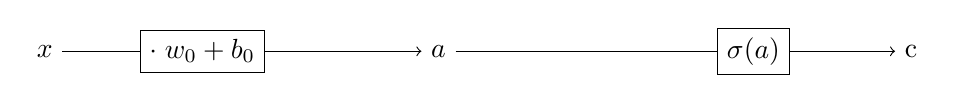
\begin{tikzpicture}
    \node (a) at (1,0) {$x$};
    \node (b) at (6,0) {$a$};
    \node (c) at (12,0) {c};
    \node[draw] (box1) at (3,0) {$\cdot\; w_0 + b_0$}; 
    \node[draw] (box2) at (10,0) {$\sigma(a)$};
    \draw[-] (a) -- (box1);
    \draw[->] (box1) -- (b); 
    \draw[-] (b) -- (box2);
    \draw[->] (box2) -- (c);
\end{tikzpicture}
\end{document}
